\chapter{Run 3 Luminosity Measurement}  %Title of the First Chapter

\ifpdf
    \graphicspath{{Chapter1/Figs/Raster/}{Chapter1/Figs/PDF/}{Chapter1/Figs/}}
\else
    \graphicspath{{Chapter1/Figs/Vector/}{Chapter1/Figs/}}
\fi

%\section{Systematic uncertainty in PCC luminosity measurement}
%\label{sec:sysunc}


%Please ask Luis for latest 2022 calibration plots

%module veto plots are in slides from Antonio in December PCC meeting

%Afterglow residuals are in my slides in PCC meeting  January , February 


%Chapter 5: Run 3 Luminosity Measurement 

%Detector Module selection
%Afterglow Model- Detector Module selection
%vdM Calibration Results
%Luminosity for Physics Fills
%Systematic Uncertainties


\section{Detector Module selection}


\begin{figure}[!htp]
\centering
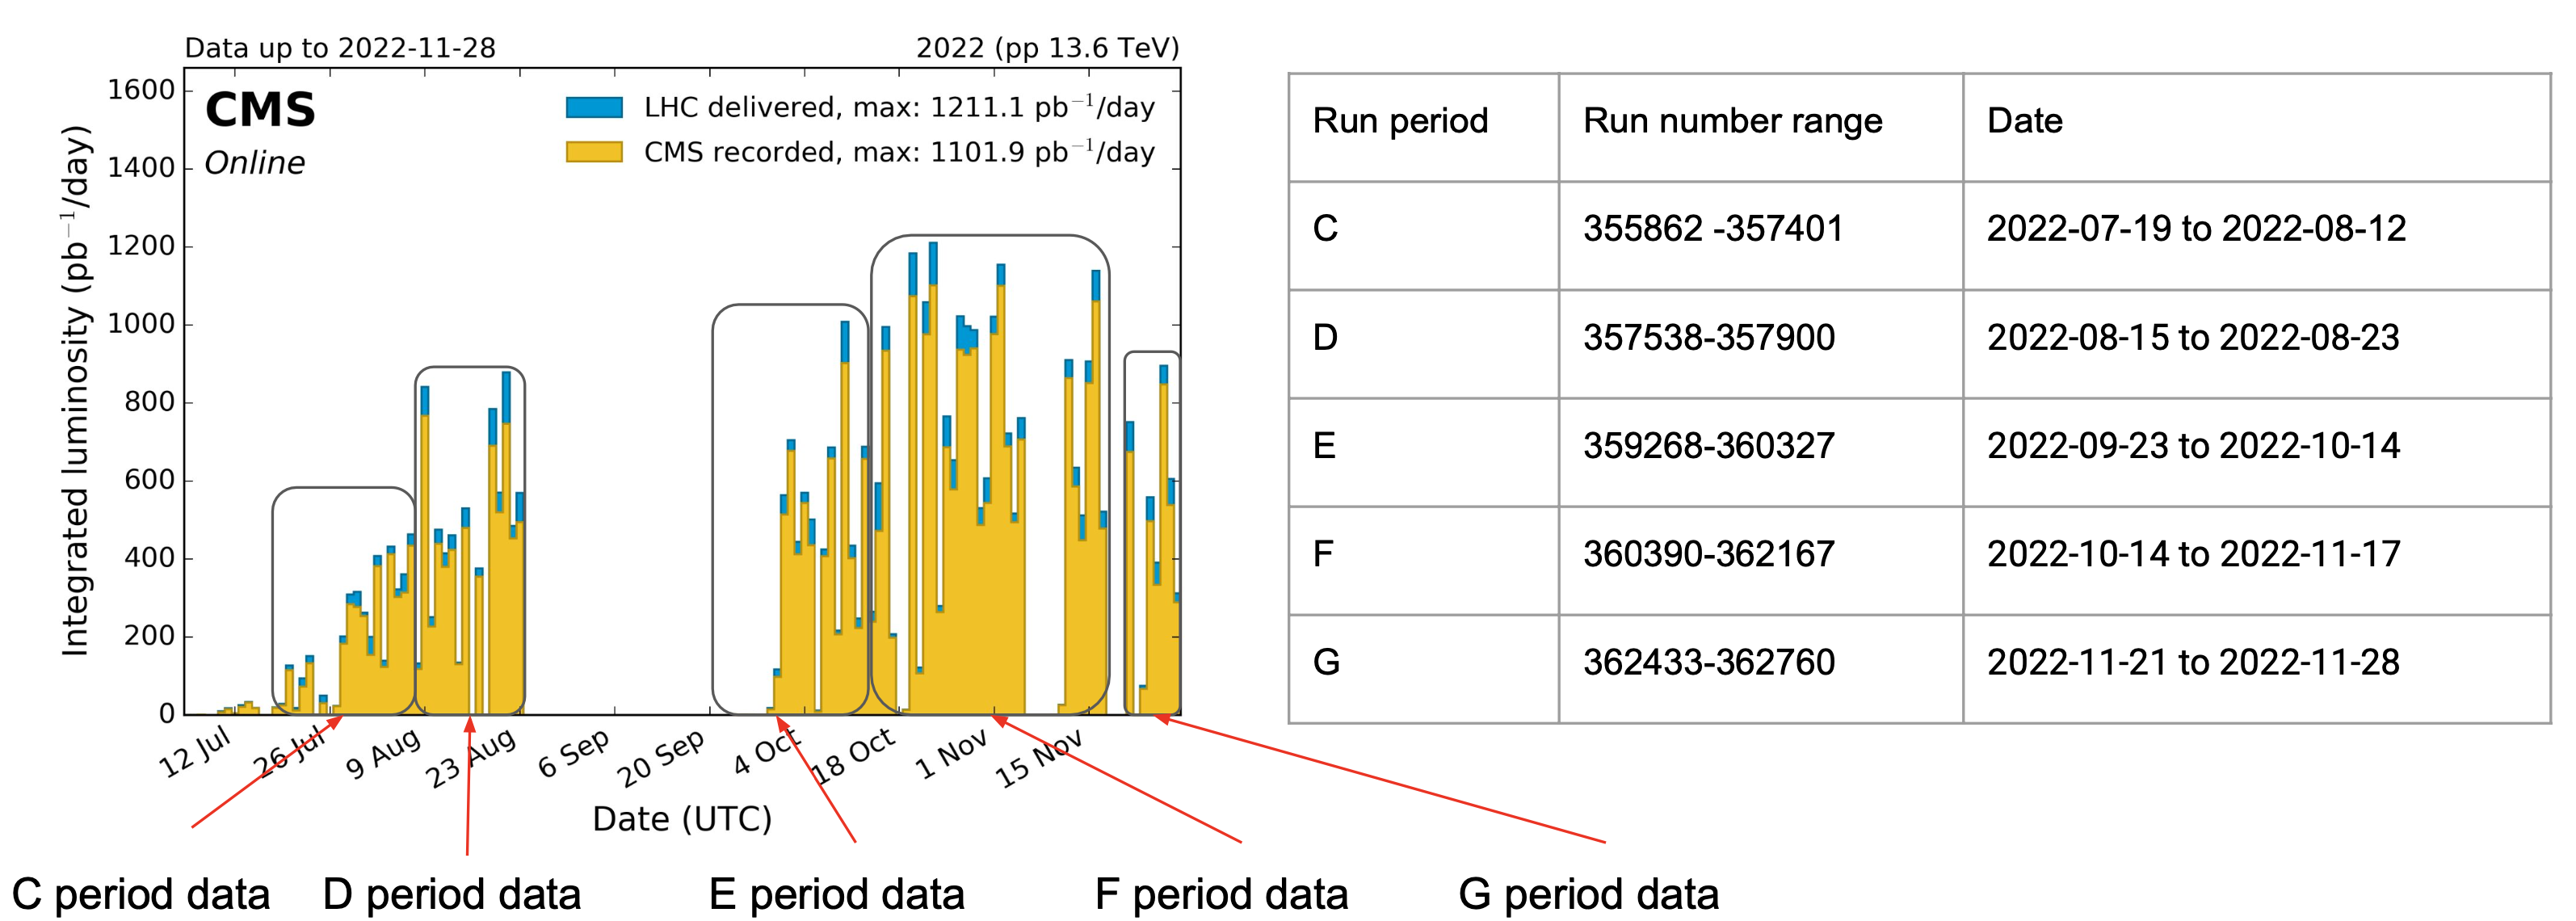
\includegraphics[width=1\textwidth]{ashish_thesis/2022_dataset.png}
\caption[2018 CMS luminosity data taking periods.]{%                                                                                                                                              
   2022 luminosity data taking periods showing data taking period boundaries and vdM calibration data  \cite{CERNLumiPublicResults}.
}
\label{fig:period_bound}
\end{figure}



\begin{figure}[!htp]
\centering
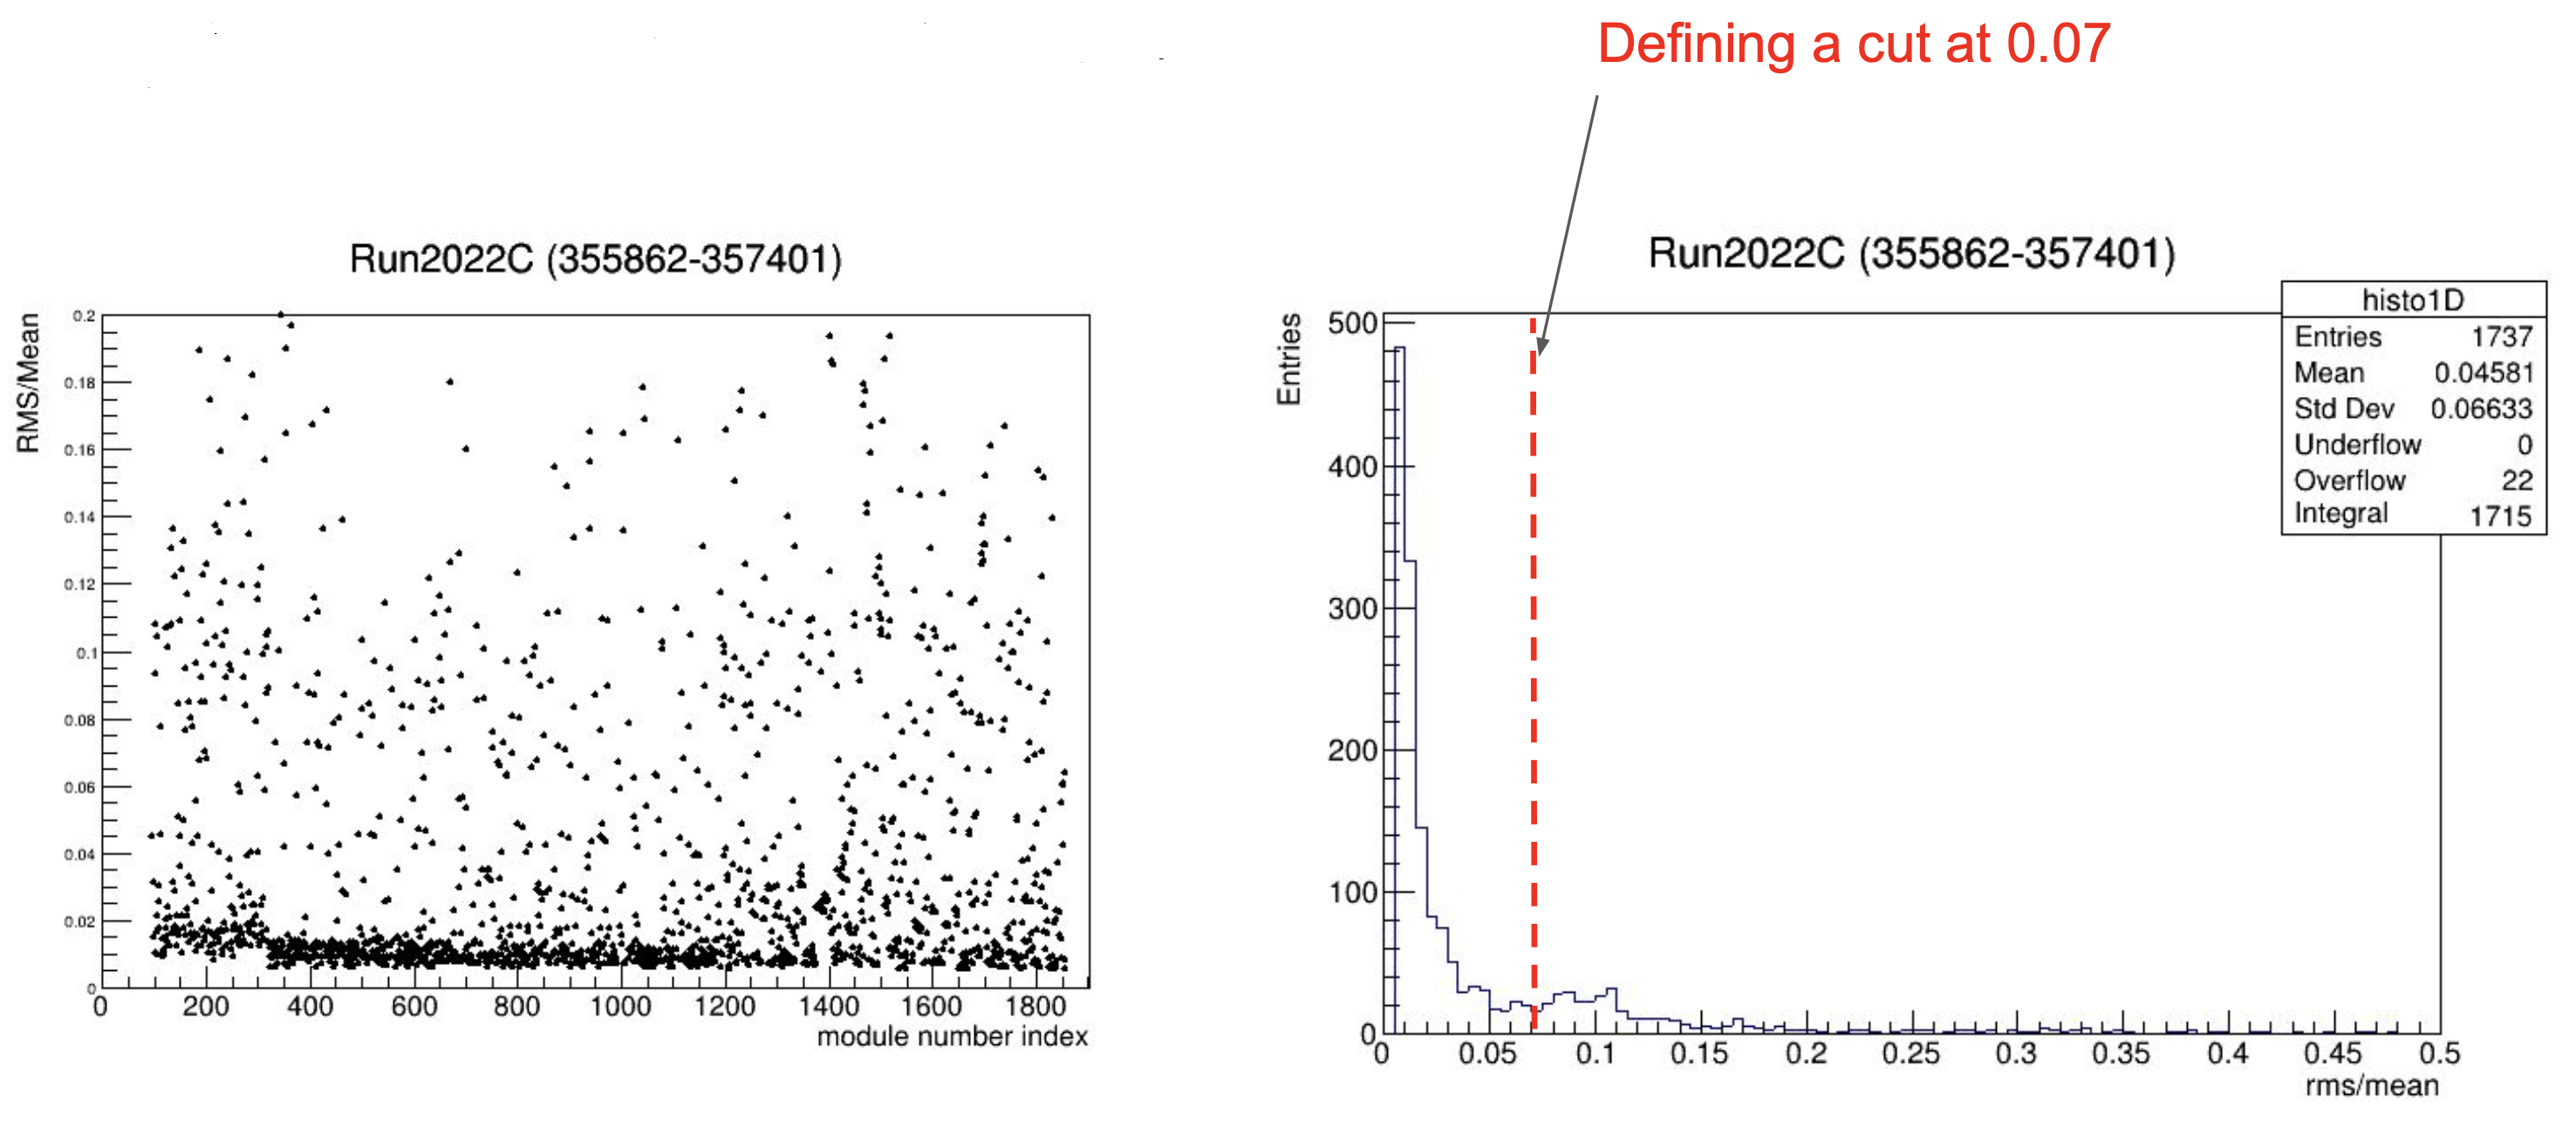
\includegraphics[width=1\textwidth]{ashish_thesis/2022_periodC_first_iteration}
\caption[2018 CMS luminosity data taking periods.]{%
  2022 luminosity data taking periods showing data taking period boundaries and vdM calibration data  \cite{CERNLumiPublicResults}.
}
\label{fig:period_bound}
\end{figure}





\begin{figure}[!htp]
\centering
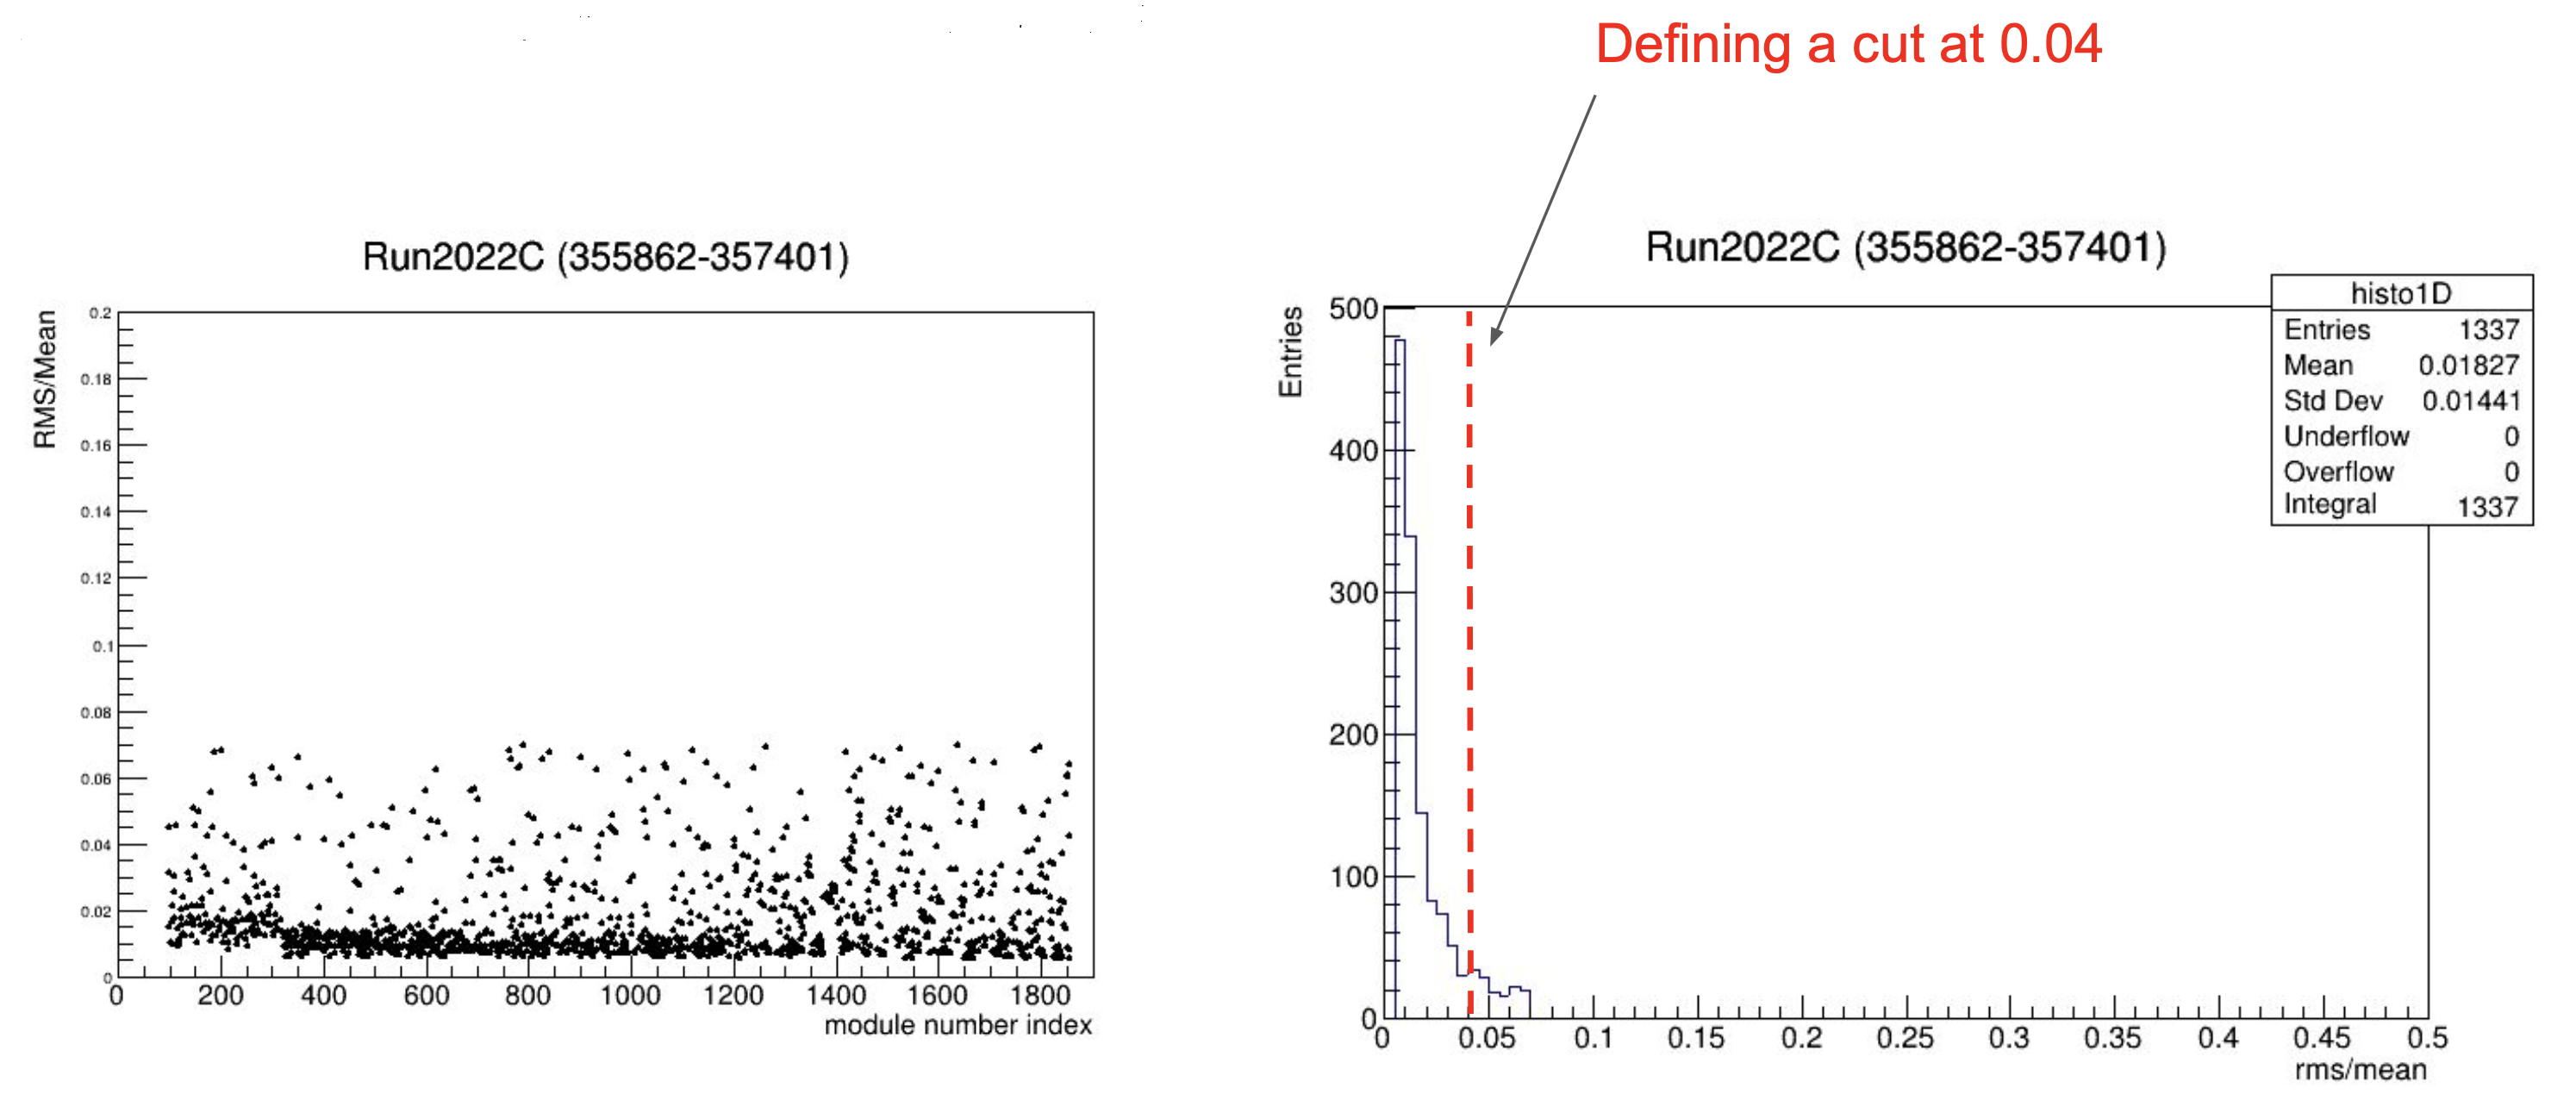
\includegraphics[width=1\textwidth]{ashish_thesis/2022_periodC_final_iteration.png}
\caption[2018 CMS luminosity data taking periods.]{%                                                                                                                                              
  2022 luminosity data taking periods showing data taking period boundaries and vdM calibration data  \cite{CERNLumiPublicResults}.
}
\label{fig:period_bound}
\end{figure}







\begin{figure}[!htp]
\centering
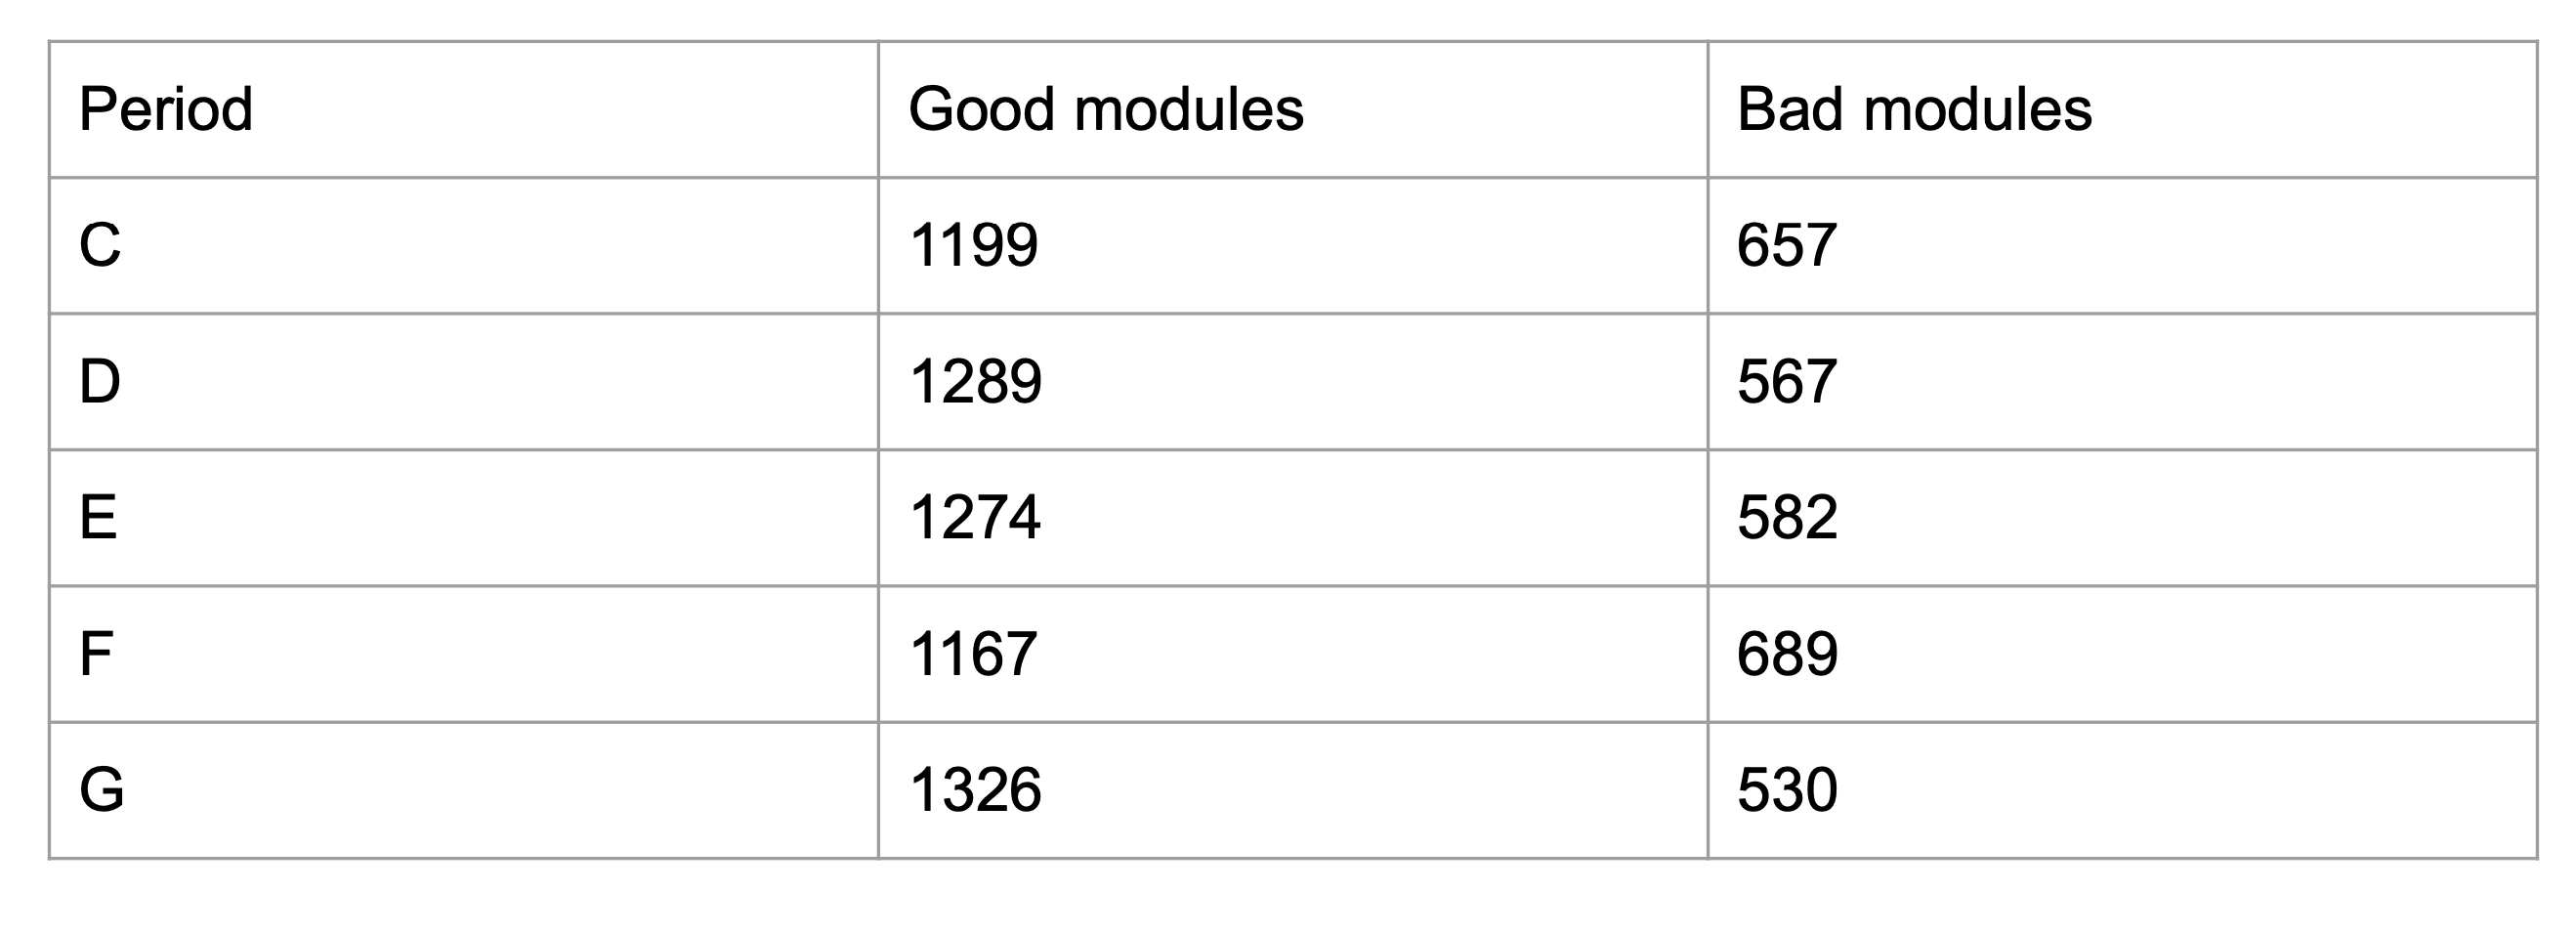
\includegraphics[width=1\textwidth]{ashish_thesis/2022_per_period_veto.png}
\caption[2018 CMS luminosity data taking periods.]{%                                                                                                                                         
  2022 luminosity data taking periods showing data taking period boundaries and vdM calibration data  \cite{CERNLumiPublicResults}.
}
\label{fig:period_bound}
\end{figure}








\begin{figure}[!htp]
\centering
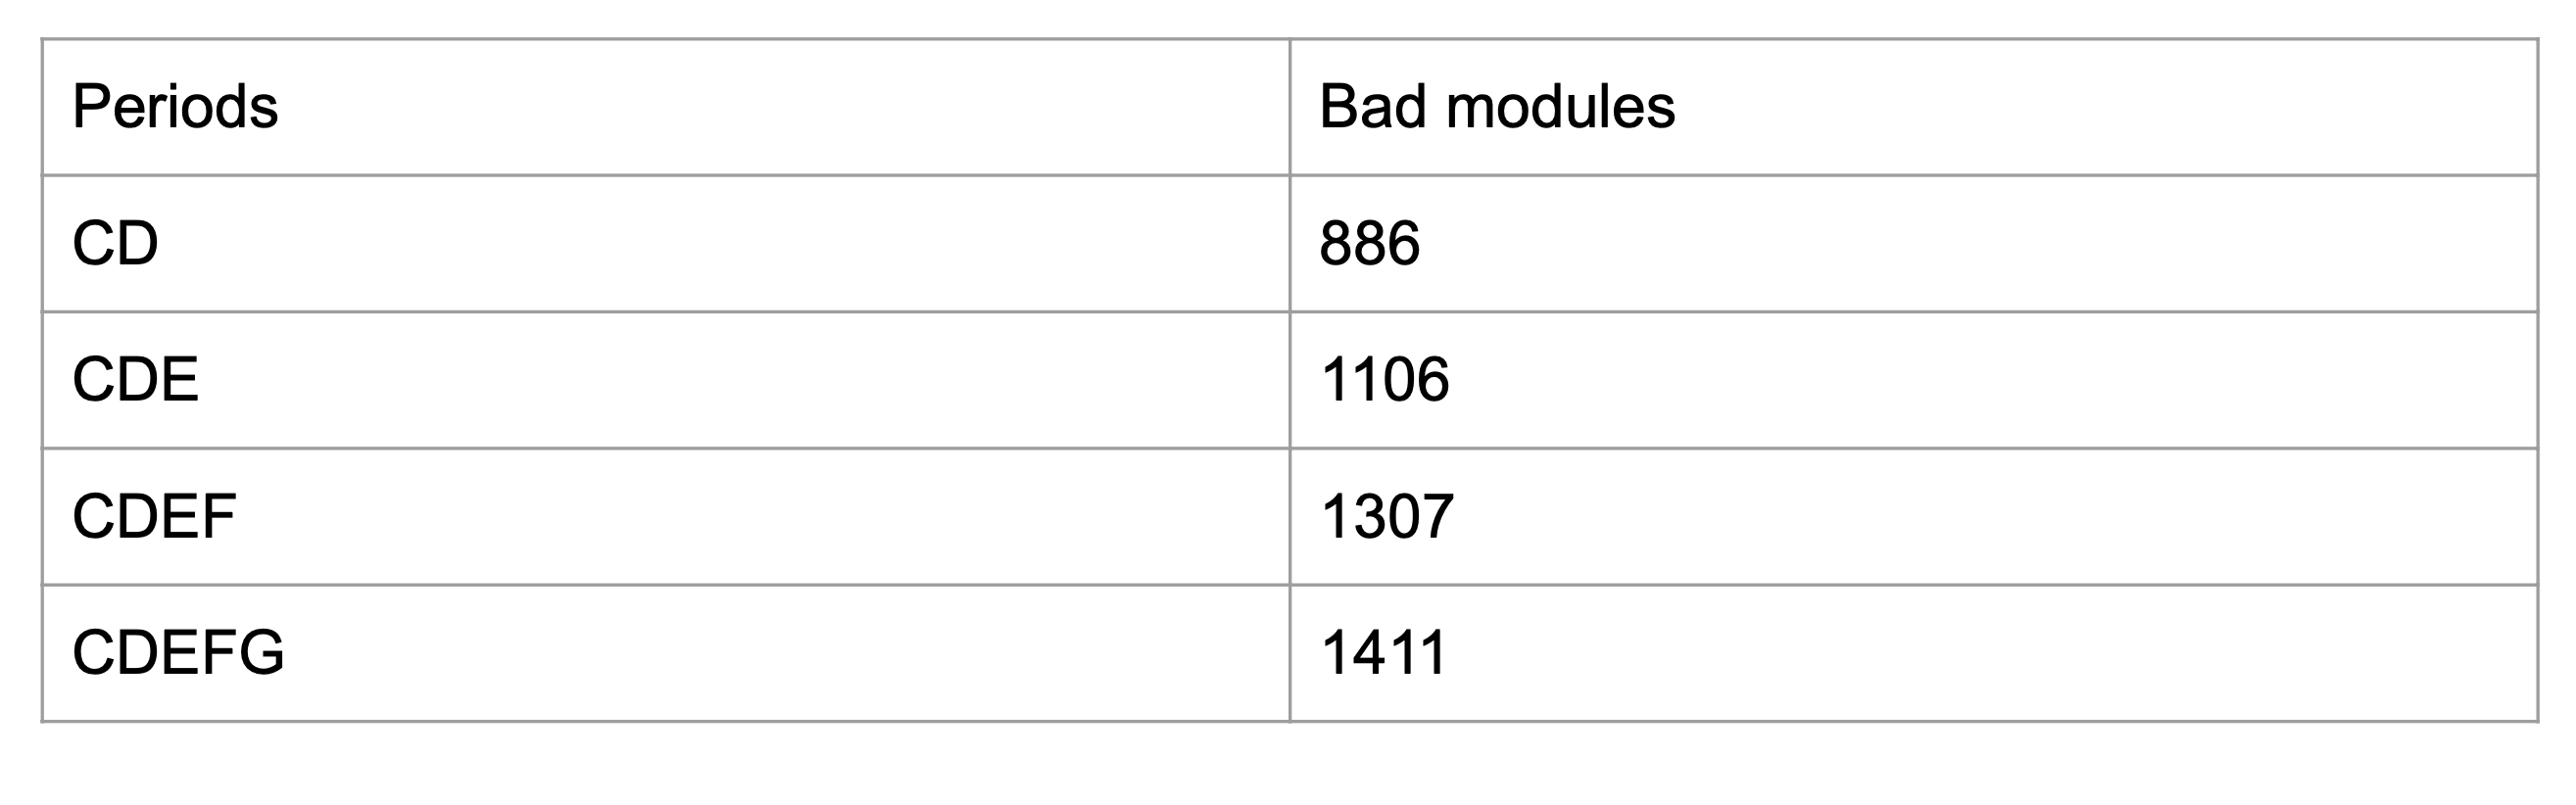
\includegraphics[width=1\textwidth]{ashish_thesis/2022_common_veto.png}
\caption[2018 CMS luminosity data taking periods.]{%                                                                                                                                             
  2022 luminosity data taking periods showing data taking period boundaries and vdM calibration data  \cite{CERNLumiPublicResults}.
}
\label{fig:period_bound}
\end{figure}




\section{Afterglow Model}



\begin{figure}[!htp]
\centering
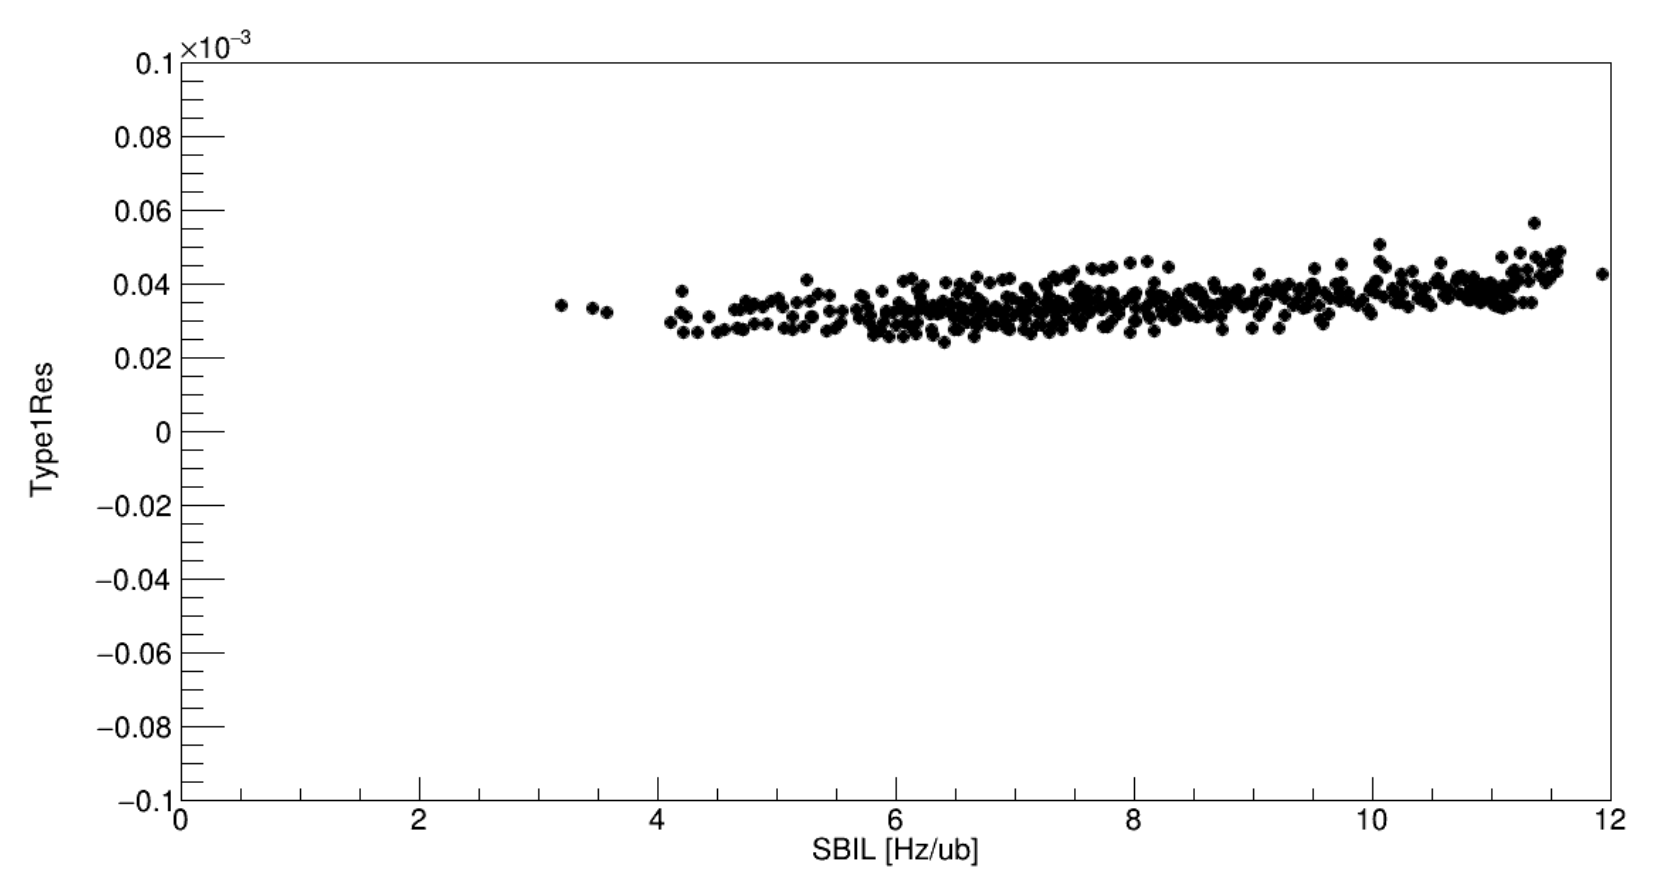
\includegraphics[width=1\textwidth]{ashish_thesis/2022_type1res.png}
\caption[2018 CMS luminosity data taking periods.]{%                                                                                                                                             
  2022 luminosity data taking periods showing data taking period boundaries and vdM calibration data  \cite{CERNLumiPublicResults}.
}
\label{fig:period_bound}
\end{figure}



\begin{figure}[!htp]
\centering
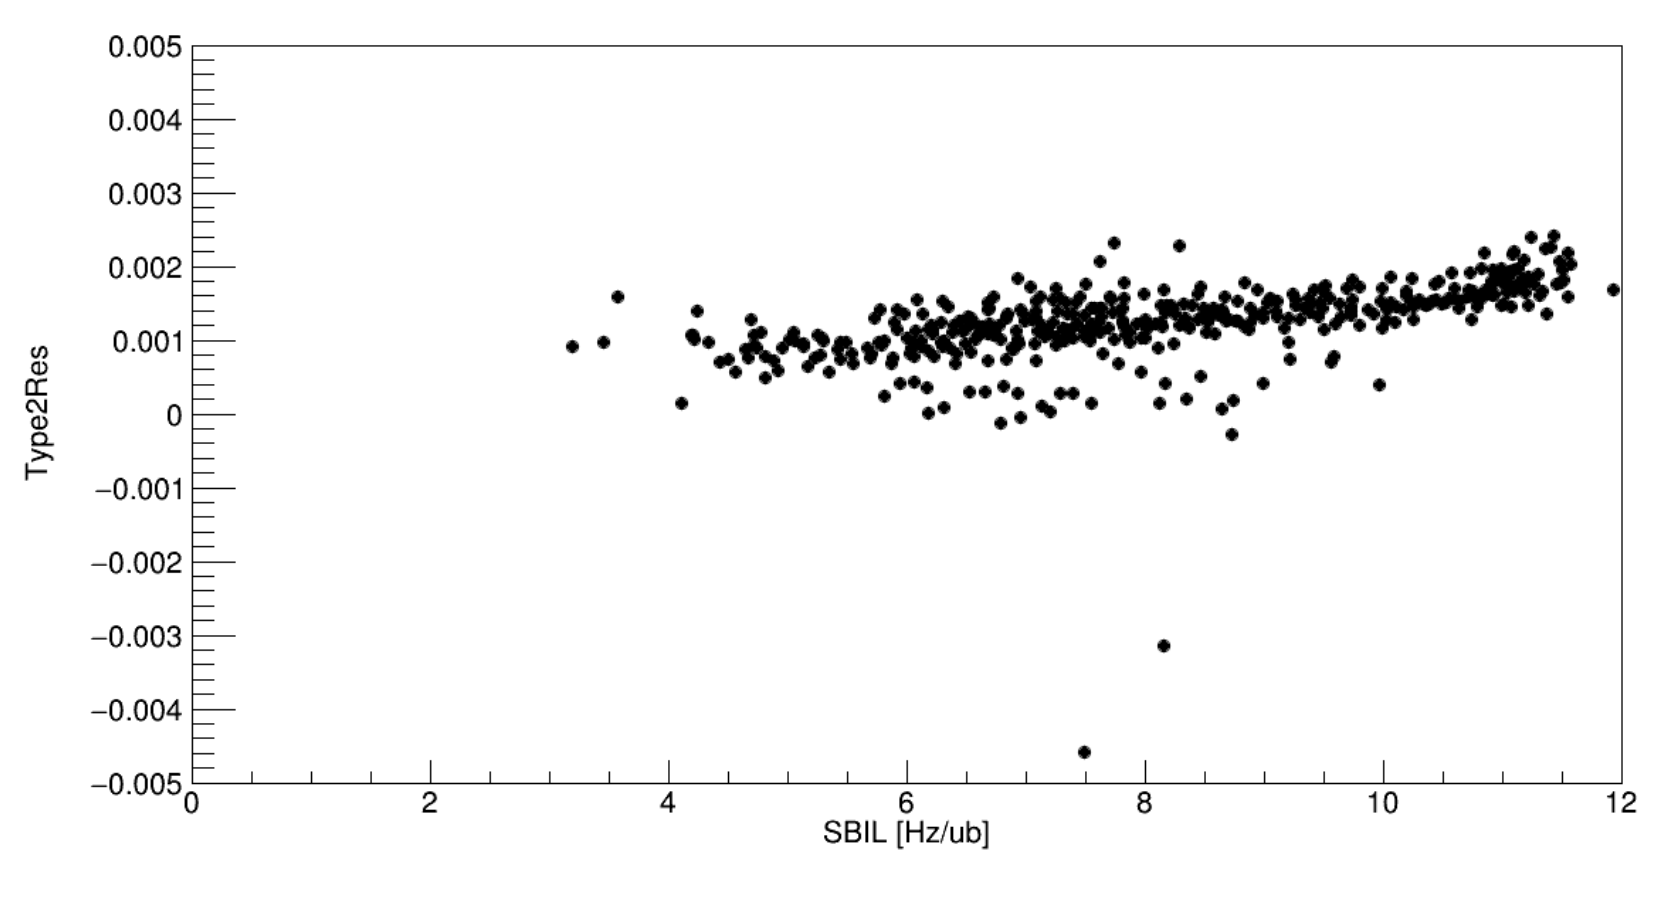
\includegraphics[width=1\textwidth]{ashish_thesis/2022_type2res.png}
\caption[2018 CMS luminosity data taking periods.]{%                                                                                                                                             
  2022 luminosity data taking periods showing data taking period boundaries and vdM calibration data  \cite{CERNLumiPublicResults}.
}
\label{fig:period_bound}
\end{figure}










\section{vdM Calibration Results}

\begin{figure}[!htp]
\centering
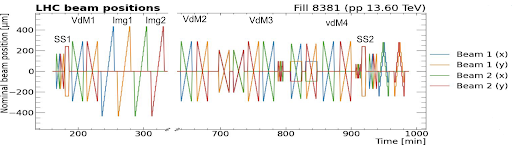
\includegraphics[width=1\textwidth]{ashish_thesis/2022_vdM.png}
\caption[2018 CMS luminosity data taking periods.]{%                                                                                                                                             
  2022 luminosity data taking periods showing data taking period boundaries and vdM calibration data  \cite{CERNLumiPublicResults}.
}
\label{fig:period_bound}
\end{figure}






\begin{figure}[!htp]
\centering
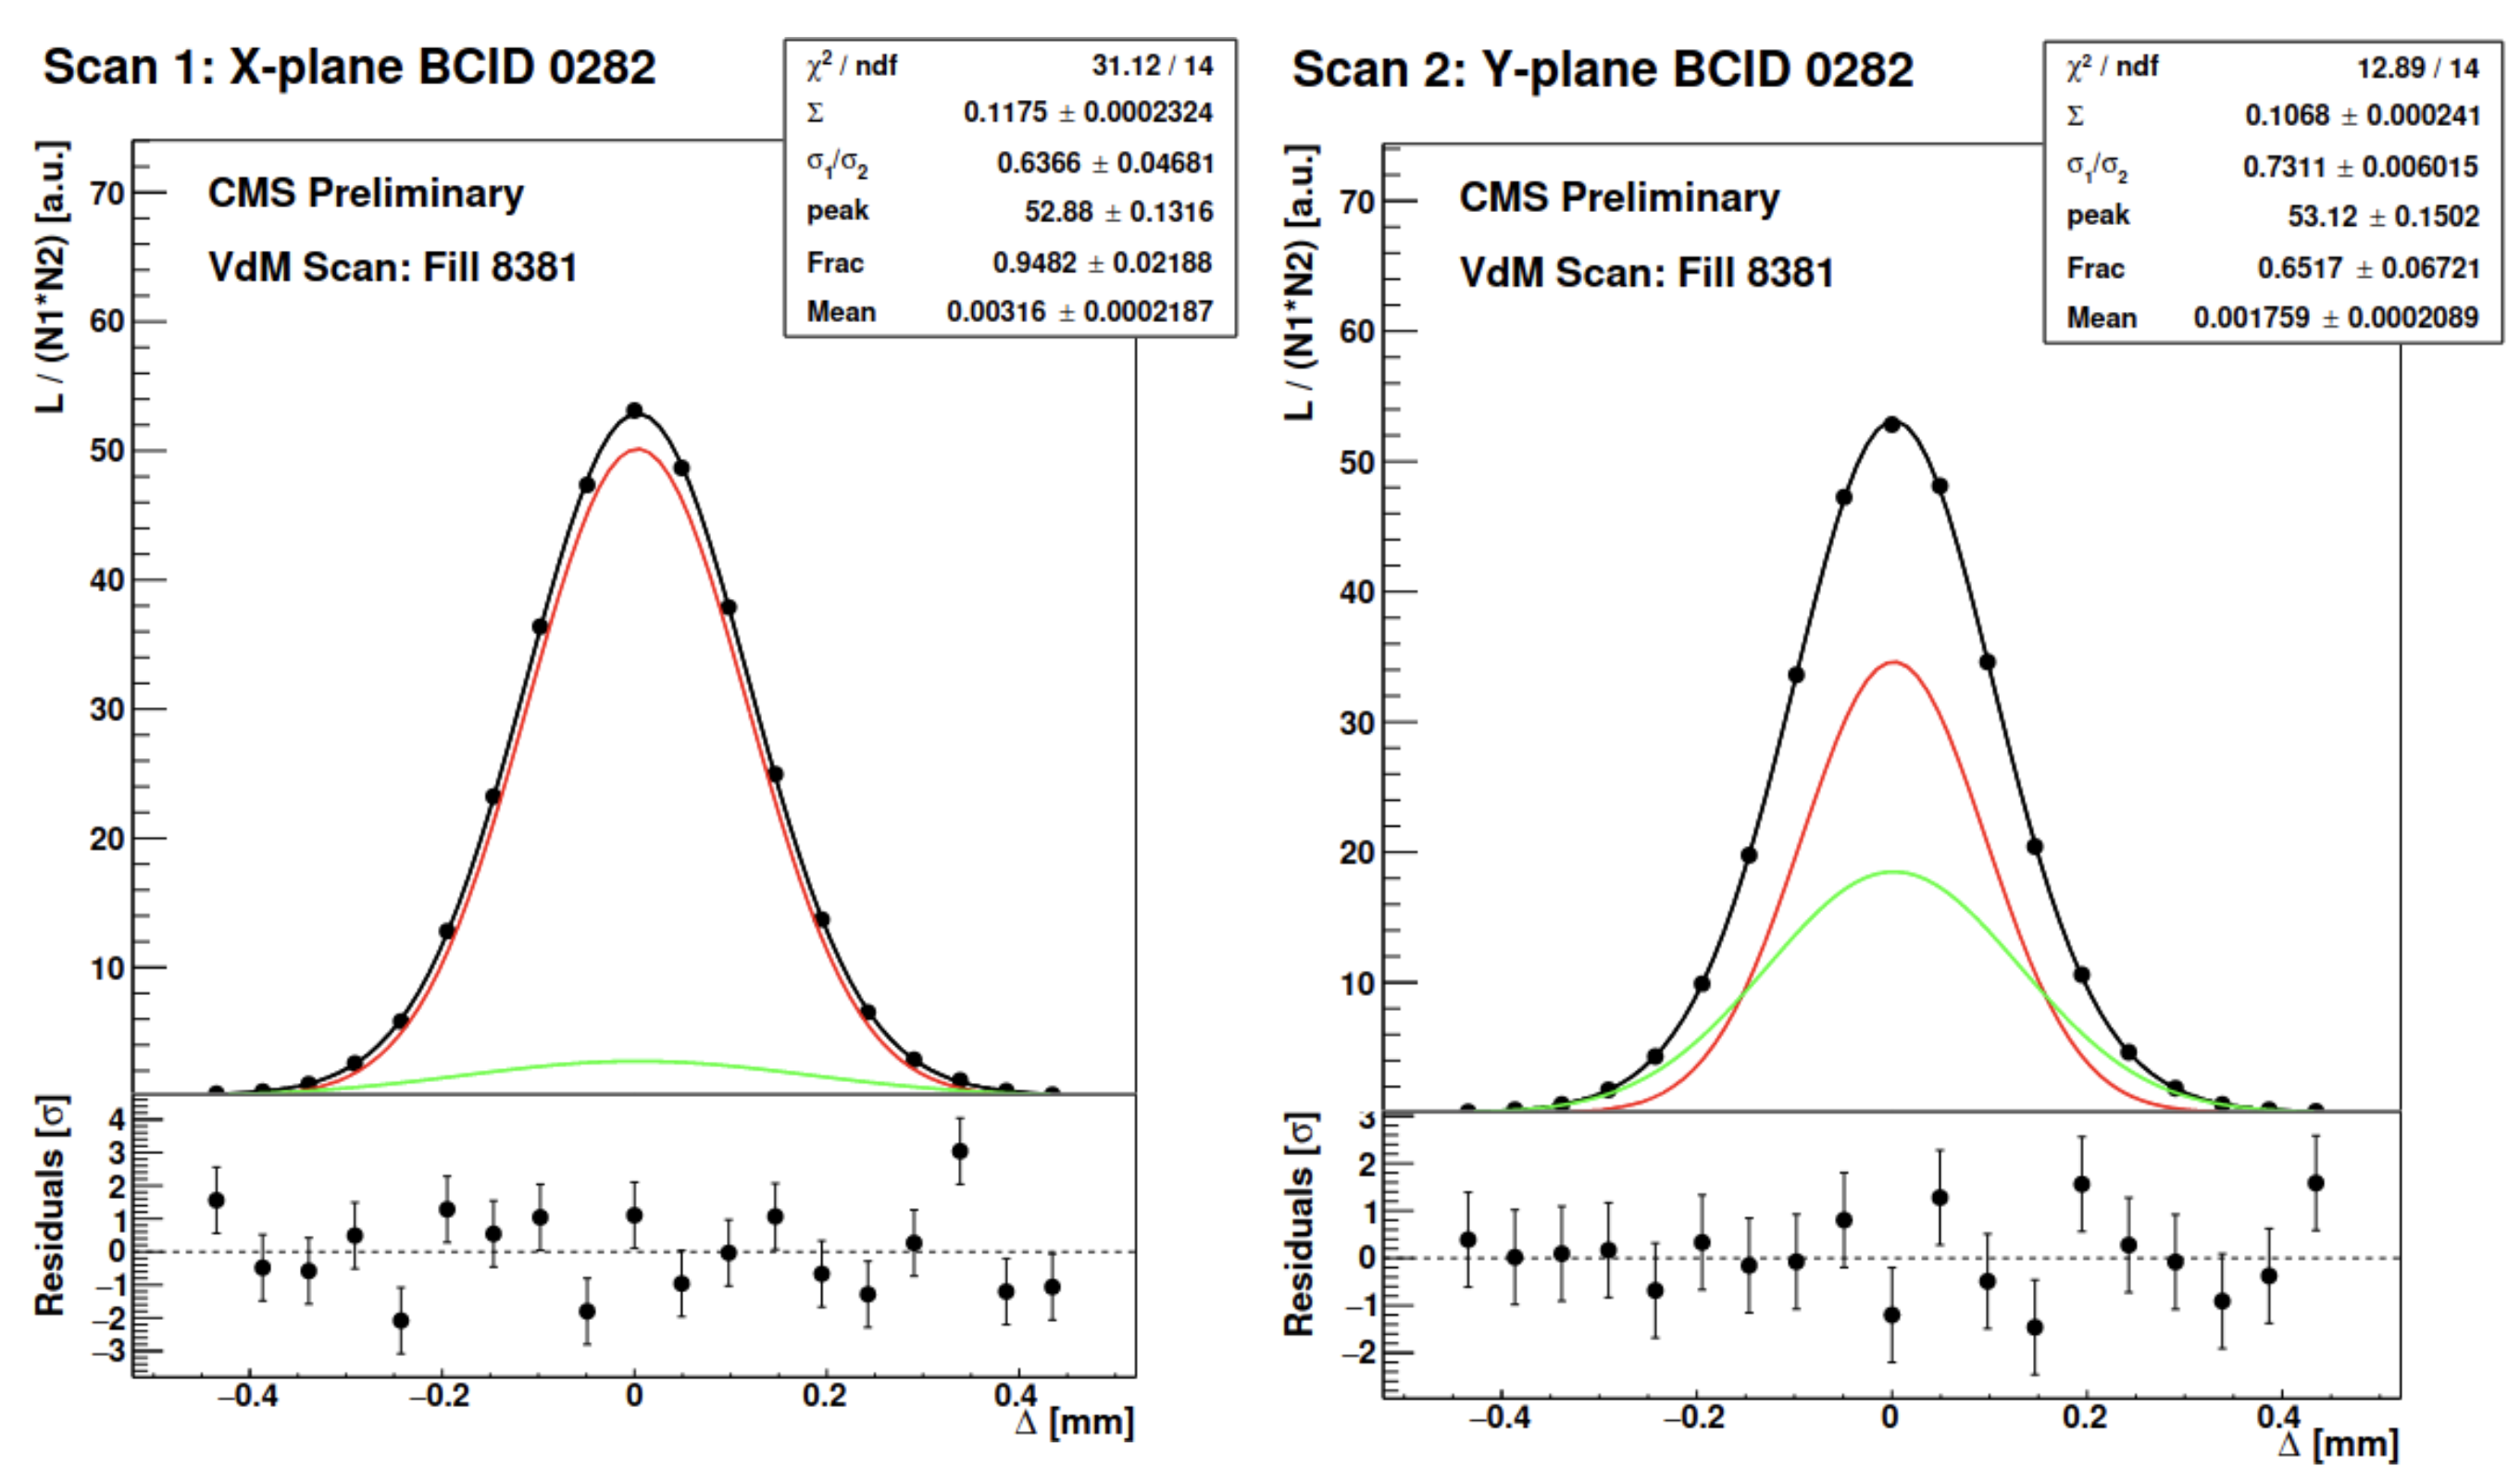
\includegraphics[width=1\textwidth]{ashish_thesis/2022_vdM_fit.png}
\caption[2018 CMS luminosity data taking periods.]{%                                                                                                                                              
  2022 luminosity data taking periods showing data taking period boundaries and vdM calibration data  \cite{CERNLumiPublicResults}.
}
\label{fig:period_bound}
\end{figure}



\begin{figure}[!htp]
\centering
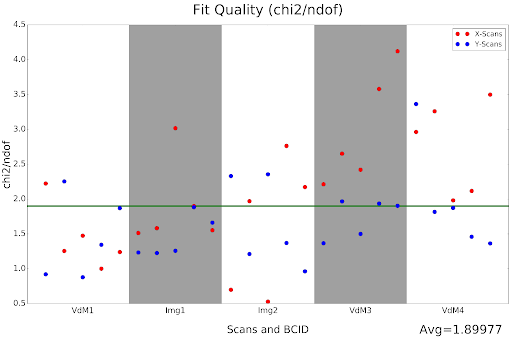
\includegraphics[width=1\textwidth]{ashish_thesis/2022_vdM_fit_quality-png.png}
\caption[2018 CMS luminosity data taking periods.]{%                                                                                                                                             
  2022 luminosity data taking periods showing data taking period boundaries and vdM calibration data  \cite{CERNLumiPublicResults}.
}
\label{fig:period_bound}
\end{figure}



\begin{figure}[!htp]
\centering
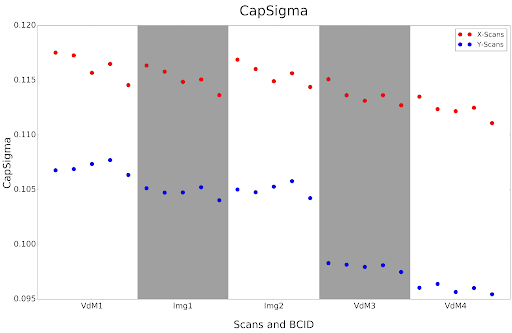
\includegraphics[width=1\textwidth]{ashish_thesis/2022_capsigma.png}
\caption[2018 CMS luminosity data taking periods.]{%                                                                                                                                             
  2022 luminosity data taking periods showing data taking period boundaries and vdM calibration data  \cite{CERNLumiPublicResults}.
}
\label{fig:period_bound}
\end{figure}






\begin{figure}[!htp]
\centering
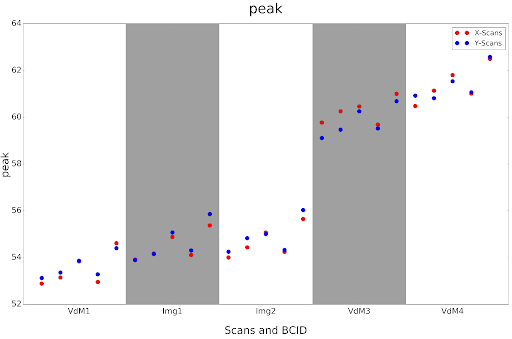
\includegraphics[width=1\textwidth]{ashish_thesis/2022_peak.png}
\caption[2018 CMS luminosity data taking periods.]{%                                                                                                                                             
  2022 luminosity data taking periods showing data taking period boundaries and vdM calibration data  \cite{CERNLumiPublicResults}.
}
\label{fig:period_bound}
\end{figure}






\begin{figure}[!htp]
\centering
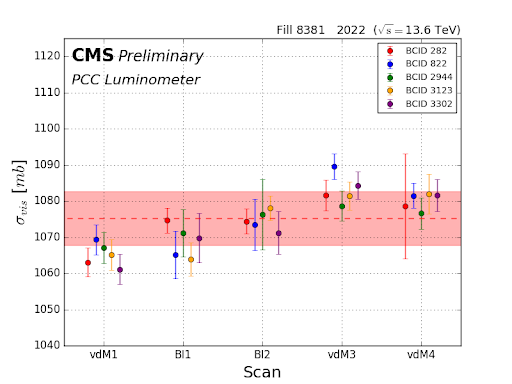
\includegraphics[width=1\textwidth]{ashish_thesis/2022_sigma_vis_btob_variation.png}
\caption[2018 CMS luminosity data taking periods.]{%                                                                                                                                             
  2022 luminosity data taking periods showing data taking period boundaries and vdM calibration data  \cite{CERNLumiPublicResults}.
}
\label{fig:period_bound}
\end{figure}







\begin{figure}[!htp]
\centering
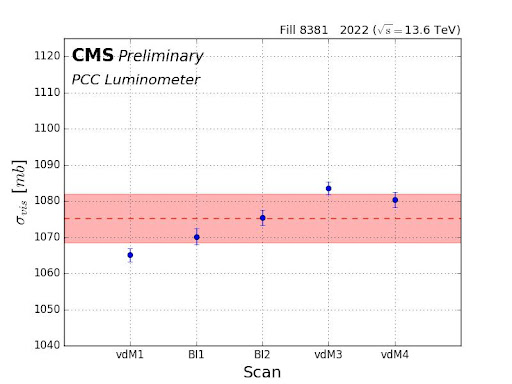
\includegraphics[width=1\textwidth]{ashish_thesis/2022_sigma_vis_per_scan.png}
\caption[2018 CMS luminosity data taking periods.]{%                                                                                              
  2022 luminosity data taking periods showing data taking period boundaries and vdM calibration data  \cite{CERNLumiPublicResults}.
}
\label{fig:period_bound}
\end{figure}



Sigma Vis =  4.1694 +- 0.002 (stat) Barns
0.06\% statistical error




\section{Luminosity for Physics Fills}










\section{Systematic uncertainties}



\begin{figure}[!htp]
\centering
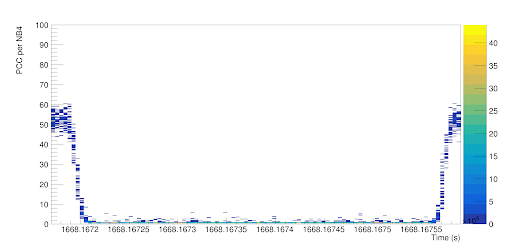
\includegraphics[width=1\textwidth]{ashish_thesis/2022_SS_scan.png}
\caption[2018 CMS luminosity data taking periods.]{%                                                                                                                                              
  2022 luminosity data taking periods showing data taking period boundaries and vdM calibration data  \cite{CERNLumiPublicResults}.
}
\label{fig:period_bound}
\end{figure}


\begin{table}[h]
    \centering
    \begin{minipage}{0.45\textwidth}
        \centering
        \caption{SS1   SS1_avg= 0.76804 +- 0.002478}
        \begin{tabular}{ccc}
        \textbf{BCID} & \textbf{Mean} & \textbf{SEM} \\ 
        \hline
        282 & .7734 & .00570 \\ 
        822 & .7756 & .00578 \\ 
        2944 & .7703 & .00599 \\ 
        3123 & .7478 & .00505 \\ 
        3302 & .7731 & .00521 \\ 
        \end{tabular}
    \end{minipage}
    \hfill
    \begin{minipage}{0.45\textwidth}
        \centering
        \caption{SS2.  SS2_avg= 0.72026 -+0.002888}
        \begin{tabular}{ccc}
        \textbf{BCID} & \textbf{Mean} & \textbf{SEM} \\ 
        \hline
        282 & .7207 & .00521 \\ 
        822 & .7247 & .00898 \\ 
        2944 & .7306 & .00616 \\ 
        3123 & .7038 & .00563 \\ 
        3302 & .7215 & .00560 \\ 
        \end{tabular}
    \end{minipage}
\end{table}



SS bkg= 0.74415 +- 0.002683










\begin{comment}

\section{Uncertainties associated with the Van der Meer calibration}

\begin{itemize}
    
\item Orbit Drift: Refers to the gradual displacement of the beam orbit from its ideal trajectory due to various effects such as ground motion, magnetic field fluctuations, and thermal expansion. This can result in reduced beam intensity and beam quality.

\item X-Y Nonfactorization: Refers to the failure of the x and y coordinates of a particle beam to factorize, meaning that the beam profile cannot be expressed as a product of independent x and y profiles. This can result in beam asymmetries and other effects.

\item Beam-Beam Deflection: Refers to the mutual interaction of two colliding particle beams, resulting in the deflection of the individual beams due to the electromagnetic fields generated by the other beam. This effect can lead to beam losses and reduced luminosity.

\item Dynamic $\beta$: Refers to the time-varying beta function of a particle beam, which describes the rate at which the beam diverges or converges as it propagates. This effect can be important for beam stability and the control of beam emittance.

\item Beam Current Calibration: Refers to the process of accurately measuring the current of a particle beam, which is essential for many beam diagnostics and control systems.

\item Ghosts and Satellites: Refers to unwanted signals in a detector or measurement system that can arise from various sources such as scattered radiation, electronic noise, or interference from other particles. These can lead to inaccurate measurements and reduced data quality.

\item Scan to Scan Variation: Refers to the variation in experimental results obtained from different scans or measurements, which can arise from various sources such as statistical fluctuations, instrument drift, or systematic errors.

\item Bunch to Bunch Variation: Refers to the variation in the properties of individual particle bunches within a beam, such as their intensity, energy spread, or emittance. This effect can be important for beam tuning and optimization.

\item Cross-Detector Consistency: Refers to the agreement between measurements obtained from different detectors or measurement systems. This is important for verifying the accuracy and reliability of experimental results.

\item Background Subtraction: Refers to the process of removing unwanted signals from a measurement or detector system that arise from sources other than the physical phenomenon of interest, such as noise, cosmic rays, or other particles. This is essential for obtaining accurate measurements of the physical signal.

\end{itemize}

\section{Uncertainties associated with physics data taking}

\begin{itemize}

\item Stability: The CMS pixel detector is a complex instrument with many components, including silicon sensors and readout electronics, that must operate consistently and with high precision over long periods. Any variations in the performance of the detector can affect the efficiency of the pixel cluster counting method and lead to uncertainties in the luminosity measurement.

One example of how the stability of the detector can affect the luminosity measurement is through changes in the detector's noise level. The noise level refers to the level of electronic noise present in the detector, which can interfere with the detection of pixel clusters produced by proton-proton collisions. If the noise level increases, the efficiency of the pixel cluster counting method may decrease, leading to an underestimation of the luminosity. Conversely, if the noise level decreases, the efficiency of the method may increase, leading to an overestimation of the luminosity.

Another example is changes in the efficiency of the pixel detector. The efficiency of the detector refers to the fraction of proton-proton collisions that produce pixel clusters that can be detected and counted by the method. Any changes in the efficiency of the detector, for example due to changes in the gain or response of the silicon sensors, can lead to uncertainties in the luminosity measurement.

To mitigate these uncertainties, the CMS collaboration performs regular calibrations and monitoring of the detector performance, as well as cross-checks with other luminosity measurement techniques

Systematic uncertainties due to stability in the detector itself for the pixel cluster counting method are typically estimated by studying the performance of the method over time and comparing it to simulations or other measurements. Uncertainties due to changes in the noise level and detector efficiency are typically estimated separately and combined to obtain the total systematic uncertainty

\item Linearity: the luminosity obtained from the PCC method is compared to that obtained from the HFOC method for a given set of collisions. Any deviations between the two measurements are used to estimate the linearity uncertainty in the PCC method.

The linearity uncertainty is typically quantified as a systematic uncertainty in the luminosity measurement, expressed as a percentage of the measured luminosity. This uncertainty can be estimated by fitting the PCC and HFOC measurements to a linear function and calculating the deviation of the PCC measurement from the linear fit.

\item Type 1 afterglow refers to the persistence of charge in the pixels of the detector after a collision event. This charge can be produced by various sources, such as ionization due to the passage of charged particles, or leakage currents in the readout electronics. If this charge is not properly accounted for, it can be mistakenly counted as pixel clusters produced by subsequent collision events, leading to an overestimation of the luminosity.

Type 2 afterglow refers to the persistence of noise in the detector after a collision event. This noise can be produced by various sources, such as thermal or radiation-induced effects, and can also interfere with subsequent collisions. If this noise is not properly accounted for, it can lead to a reduction in the efficiency of the pixel cluster counting method and an underestimation of the luminosity.

\end{itemize}



\section{Comparison of PCC with HFOC luminosity}

\end{comment}
